\section{Grundlagen}

Dieses Kapitel stellt die theoretischen und technischen Grundlagen vor, die zum Verständnis der akustischen Time-of-Flight-Messung im Außenbereich erforderlich sind.

\subsection{Schallausbreitung im Außenraum}

Die Ausbreitung von Schallwellen im Außenraum wird maßgeblich durch die physikalischen Eigenschaften der Luft sowie durch Umwelteinflüsse bestimmt. Die Schallgeschwindigkeit $c$ in trockener Luft lässt sich näherungsweise in Abhängigkeit von der Lufttemperatur $T$ in Grad Celsius durch die Beziehung
\[
c \approx 331{,}3 \, \text{m/s} + 0{,}6 \cdot T \, \text{m/s}
\]
beschreiben \cite{kuttruff2000raumakustik}. Temperaturänderungen wirken sich somit direkt auf die Laufzeitmessungen aus und müssen bei präzisen Time-of-Flight-Verfahren berücksichtigt werden. Neben der Temperatur beeinflussen auch Luftfeuchtigkeit und Luftdruck die Schallgeschwindigkeit, wenngleich in geringerem Maße \cite{bass1995atmospheric}.

Ein wesentlicher Aspekt der Schallausbreitung im Freien ist die Dämpfung mit zunehmender Entfernung. Diese setzt sich aus geometrischer Ausbreitung (Kugelausbreitung) und frequenzabhängiger atmosphärischer Absorption zusammen. Während die geometrische Dämpfung mit $1/r$ (bei Druckamplituden) bzw. $1/r^2$ (bei Intensitäten) beschrieben wird, nimmt die Absorption mit steigender Frequenz deutlich zu. Dies begrenzt die Reichweite insbesondere hochfrequenter akustischer Signale.

Darüber hinaus beeinflussen Umgebungsbedingungen die Ausbreitung erheblich. Wind kann durch Geschwindigkeitsgradienten zu einer Richtungsabhängigkeit der Schallgeschwindigkeit führen, wodurch Laufzeiten verzerrt werden. Turbulenzen verursachen zusätzlich Pegelschwankungen und Phasenmodulationen \cite{salomons2001computational}. Auch Boden- und Gebäudereflexionen führen zu Mehrwegeffekten, die bei Laufzeitmessungen als systematische Störgrößen in Erscheinung treten können. Diese Effekte sind im Kontext akustischer Entfernungsmessung besonders kritisch, da sie Fehlinterpretationen bei der Korrelation verursachen können.

Für die vorliegende Arbeit sind insbesondere zwei Punkte relevant: Erstens die temperaturabhängige Variation der Schallgeschwindigkeit, die bei Messungen im Außenraum durch eine entsprechende Korrektur kompensiert werden muss. Zweitens die Beeinflussung durch Mehrwegeffekte und atmosphärisches Rauschen, welche die Detektionswahrscheinlichkeit der gesendeten Signale reduzieren und die Erkennungsrate limitieren können.


\subsection{Signalgestaltung für akustische \ac{ToF}-Verfahren}

Die Wahl des Sendesignals ist ein entscheidender Faktor für die Genauigkeit und Robustheit akustischer \ac{ToF}-Messungen. Grundsätzlich lassen sich zwei Kategorien unterscheiden: Impulssignale und kontinuierliche, modulierte Signale. Während kurze Impulse eine einfache Auswertung ermöglichen, sind sie gegenüber Störgeräuschen und Mehrwegeffekten anfälliger und bieten eine geringere Reichweite. Demgegenüber weisen frequenzmodulierte Signale, insbesondere lineare Chirp-Signale, vorteilhafte Eigenschaften auf \cite{cook1960pulse}.

Chirp-Signale zeichnen sich durch eine zeitlich lineare Änderung der Frequenz aus. Durch ihre große Zeit-Bandbreite-Produkte besitzen sie schmale Korrelationspeaks und ermöglichen somit eine präzise Laufzeitbestimmung. Gleichzeitig erlaubt ihre Energieverteilung über einen breiten Frequenzbereich eine hohe Robustheit gegenüber schmalbandigen Störungen \cite{winkler1995range}. In akustischen Anwendungen im hörbaren Frequenzbereich wird typischerweise ein Sweep von einigen Kilohertz gewählt, wobei die Auswahl durch die Übertragungscharakteristik von Lautsprecher und Mikrofon begrenzt ist.

Die Parameterwahl des Chirp-Signals stellt einen Kompromiss zwischen Reichweite und Auflösung dar. Eine größere Bandbreite erhöht die Zeitauflösung, erfordert jedoch geeignete Hardware zur Signalübertragung und -aufnahme. Eine längere Signaldauer steigert die Energie und damit die Reichweite, vergrößert jedoch auch die Anfälligkeit gegenüber Mehrwegeeffekten. Daher ist eine sorgfältige Abstimmung von Bandbreite, Dauer und Amplitude erforderlich, um unter den gegebenen Außenraumbedingungen zuverlässige Messergebnisse zu erzielen.


\subsection{Korrelationsmethoden}

Zur Bestimmung der Laufzeitdifferenz zwischen gesendetem und empfangenem Signal werden in akustischen Time-of-Flight-Systemen Korrelationsverfahren eingesetzt. Die Kreuzkorrelation erlaubt es, das empfangene Signal mit einer Referenzversion des ausgesendeten Signals zu vergleichen und den Zeitpunkt maximaler Ähnlichkeit zu bestimmen. Mathematisch wird die Kreuzkorrelation zweier diskreter Signale $x[n]$ und $y[n]$ durch
\[
R_{xy}[k] = \sum_{n} x[n] \, y[n+k]
\]
definiert \cite{oppenheim1999discrete}. Das Maximum von $R_{xy}[k]$ markiert die geschätzte Verzögerung zwischen beiden Signalen. 

Ein wesentliches Problem tritt bei periodischen oder quasi-periodischen Signalen wie reinen Sinusschwingungen auf. Da diese eine wiederkehrende Struktur besitzen, führt die Kreuzkorrelation zu mehreren gleichwertigen Maxima, wodurch keine eindeutige Laufzeitbestimmung möglich ist. Aus diesem Grund sind breitbandige Signale wie Chirps vorzuziehen, da sie in der Korrelation einen klaren, scharfen Peak erzeugen, der sich eindeutig vom Rauschhintergrund absetzt \cite{winkler1995range}.

In verrauschten Umgebungen reduziert sich der \ac{SNR}, was die Erkennung des Korrelationspeaks erschwert. Nebenmaxima können stärker hervortreten, sodass das globale Maximum nicht mehr der tatsächlichen Laufzeit entspricht. Verfahren wie die Normalisierung der Kreuzkorrelation oder die Verwendung der \ac{GCC} mit spektralen Gewichtungen erhöhen in solchen Fällen die Robustheit \cite{knapp1976generalized}. 

Ein weiteres zentrales Thema ist die Sub-Sample-Schätzung: Da die Abtastfrequenz die Zeitauflösung begrenzt, erlaubt die Interpolation des Korrelationspeaks (z. B. parabolische Anpassung der Nachbarwerte) eine genauere Laufzeitabschätzung unterhalb der Abtastperiode \cite{lyons2011understanding}.

\begin{figure}[h]
    \centering
    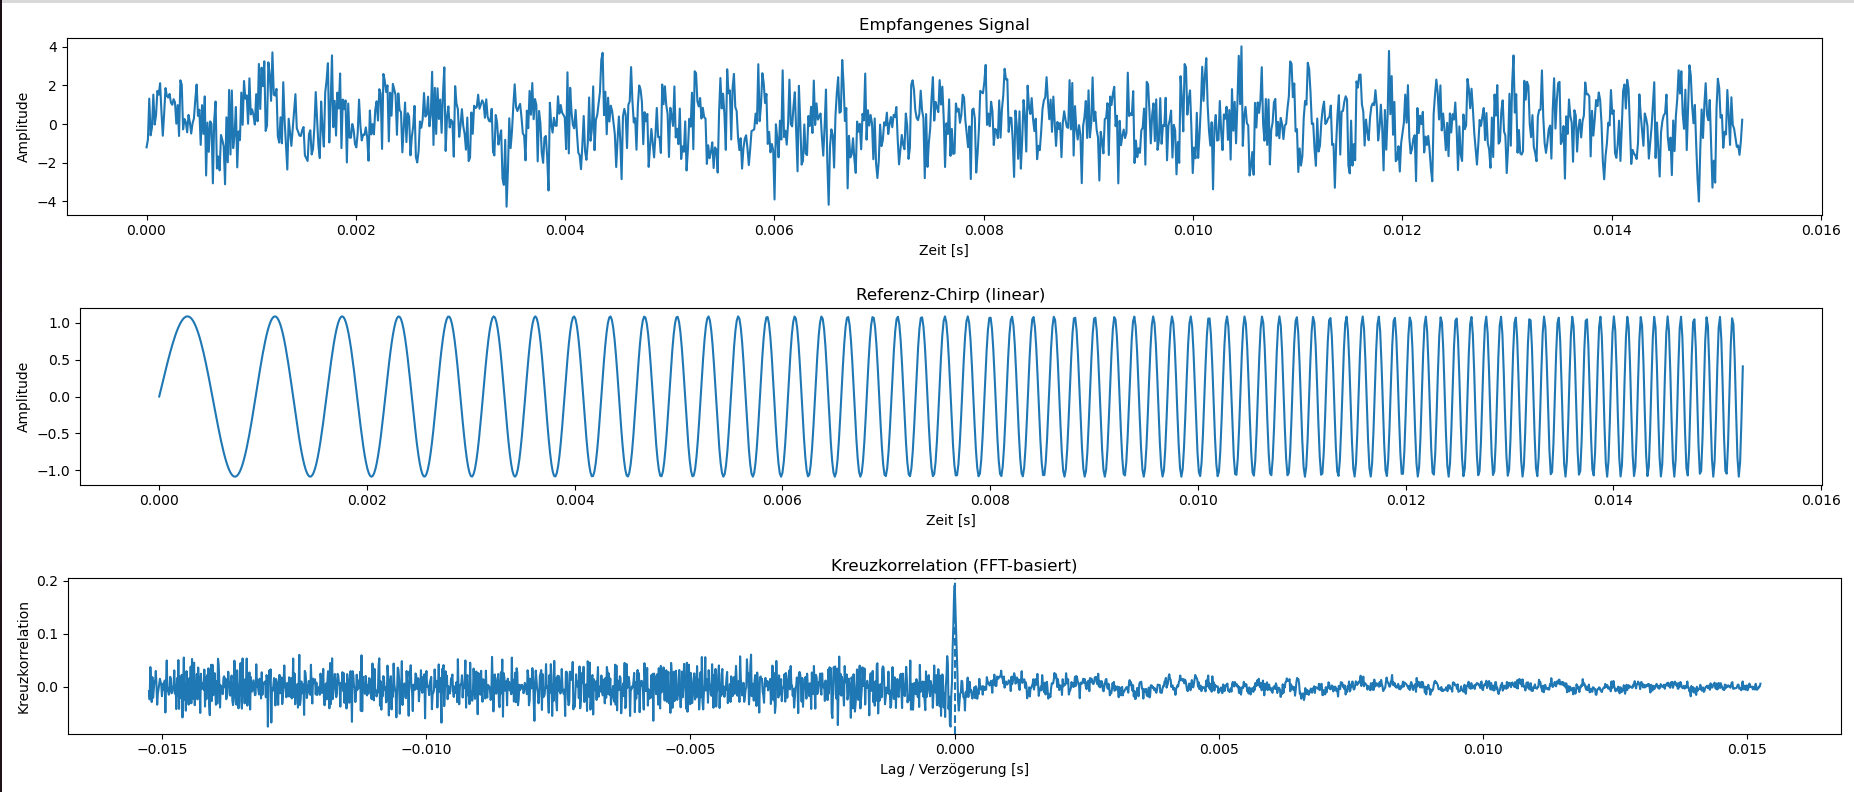
\includegraphics[width=0.9\linewidth]{korrelationsverlauf.png}
    \caption{Schematische Darstellung von Kreuzkorrelationsverläufen zur Verdeutlichung der Peak-Struktur.}
    \label{fig:correlation}
\end{figure}


\subsection{Eigenschaften von ESP32-S3 und FreeRTOS}

Der ESP32-S3 ist ein Mikrocontroller der Firma Espressif, der speziell für Anwendungen im Bereich eingebetteter Systeme mit hohen Anforderungen an Rechenleistung, Konnektivität und Energieeffizienz entwickelt wurde. Er verfügt über einen Dual-Core Xtensa LX7-Prozessor mit einer Taktfrequenz von bis zu 240\,MHz, integriertem \ac{WLAN} (\ac{IEEE} 802.11\,b/g/n) sowie \ac{Bluetooth} 5.0. Für signalverarbeitende Aufgaben stehen \ac{DSP}-Erweiterungen, Vektoroperationen sowie Hardwareunterstützung für Gleitkommazahlen zur Verfügung \cite{espressif2023esp32s3}. Darüber hinaus besitzt der ESP32-S3 dedizierte Peripherien für Audioanwendungen, wie \ac{I2S}-Schnittstellen, 12-Bit-\ac{ADC}-Kanäle und integrierte \ac{DAC}s. Dies ermöglicht die direkte Ansteuerung von \ac{MEMS}-Mikrofonen und Lautsprechern ohne zusätzliche Hardware.

Die Architektur des ESP32-S3 eignet sich für die in dieser Arbeit betrachteten akustischen \ac{ToF}-Verfahren in zweierlei Hinsicht. Erstens erlaubt die Rechenleistung die Echtzeitberechnung von Korrelationen, auch für längere Chirp-Signale und \ac{FFT}-basierte Verfahren. Zweitens unterstützt die umfangreiche Peripherie die präzise Aufnahme und Wiedergabe akustischer Signale bei Abtastraten bis 48\,kHz, wie sie für Messungen im hörbaren Frequenzbereich erforderlich sind. 

Als Betriebssystem wird FreeRTOS eingesetzt, ein weit verbreitetes Echtzeitbetriebssystem für Mikrocontroller. Es basiert auf einem präemptiven Task-Scheduler, der die Aufteilung der Rechenressourcen auf mehrere Tasks mit unterschiedlichen Prioritäten erlaubt \cite{richardbarry2022freertos}. Wichtige Mechanismen wie Queues, Semaphore und Mutexes unterstützen die Synchronisation zwischen Tasks und Interrupts. Im Kontext der akustischen Laufzeitmessung ist insbesondere die Reduktion von Jitter relevant: Durch die Zuweisung hoher Prioritäten an zeitkritische Signalverarbeitungstasks, die Verwendung von Hardware-Timern zur exakten Zeitbasis sowie das Auslagern nicht zeitkritischer Aufgaben (z.\,B. Logging, Kommunikation) auf Hintergrund-Tasks lässt sich die zeitliche Genauigkeit verbessern.

Die Kombination aus leistungsfähiger Hardware (ESP32-S3) und deterministischer Softwaresteuerung (FreeRTOS) bietet somit eine geeignete Plattform für die prototypische Realisierung akustischer Entfernungsmessungen im Außenbereich.

